\documentclass[11pt]{article}
\usepackage{float}
% NOTE: Add in the relevant information to the commands below; or, if you'll be using the same information frequently, add these commands at the top of paolo-pset.tex file. 
\newcommand{\name}{Agustín Esteva}
\newcommand{\email}{aesteva@uchicago.edu}
\newcommand{\classnum}{270}
\newcommand{\subject}{Complex Variables}
\newcommand{\instructors}{Robert Fefferman}
\newcommand{\assignment}{Problem Set 4}
\newcommand{\semester}{Spring 2025}
\newcommand{\duedate}{5-01-2025}
\newcommand{\bA}{\mathbf{A}}
\newcommand{\Ind}{\text{Ind}}

\newcommand{\bB}{\mathbf{B}}
\newcommand{\bC}{\mathbf{C}}
\newcommand{\bD}{\mathbf{D}}
\newcommand{\bE}{\mathbf{E}}
\newcommand{\bF}{\mathbf{F}}
\newcommand{\bG}{\mathbf{G}}
\newcommand{\bH}{\mathbf{H}}
\newcommand{\bI}{\mathbf{I}}
\newcommand{\bJ}{\mathbf{J}}
\newcommand{\bK}{\mathbf{K}}
\newcommand{\bL}{\mathbf{L}}
\newcommand{\bM}{\mathbf{M}}
\newcommand{\bN}{\mathbf{N}}
\newcommand{\bO}{\mathbf{O}}
\newcommand{\bP}{\mathbf{P}}
\newcommand{\bQ}{\mathbf{Q}}
\newcommand{\bR}{\mathbf{R}}
\newcommand{\bS}{\mathbf{S}}
\newcommand{\bT}{\mathbf{T}}
\newcommand{\bU}{\mathbf{U}}
\newcommand{\bV}{\mathbf{V}}
\newcommand{\bW}{\mathbf{W}}
\newcommand{\bX}{\mathbf{X}}
\newcommand{\bY}{\mathbf{Y}}
\newcommand{\bZ}{\mathbf{Z}}
\newcommand{\Vol}{\text{Vol}}

%% blackboard bold math capitals
\newcommand{\bbA}{\mathbb{A}}
\newcommand{\bbB}{\mathbb{B}}
\newcommand{\bbC}{\mathbb{C}}
\newcommand{\bbD}{\mathbb{D}}
\newcommand{\bbE}{\mathbb{E}}
\newcommand{\bbF}{\mathbb{F}}
\newcommand{\bbG}{\mathbb{G}}
\newcommand{\bbH}{\mathbb{H}}
\newcommand{\bbI}{\mathbb{I}}
\newcommand{\bbJ}{\mathbb{J}}
\newcommand{\bbK}{\mathbb{K}}
\newcommand{\bbL}{\mathbb{L}}
\newcommand{\bbM}{\mathbb{M}}
\newcommand{\bbN}{\mathbb{N}}
\newcommand{\bbO}{\mathbb{O}}
\newcommand{\bbP}{\mathbb{P}}
\newcommand{\bbQ}{\mathbb{Q}}
\newcommand{\bbR}{\mathbb{R}}
\newcommand{\bbS}{\mathbb{S}}
\newcommand{\bbT}{\mathbb{T}}
\newcommand{\bbU}{\mathbb{U}}
\newcommand{\bbV}{\mathbb{V}}
\newcommand{\bbW}{\mathbb{W}}
\newcommand{\bbX}{\mathbb{X}}
\newcommand{\bbY}{\mathbb{Y}}
\newcommand{\bbZ}{\mathbb{Z}}

%% script math capitals
\newcommand{\sA}{\mathscr{A}}
\newcommand{\sB}{\mathscr{B}}
\newcommand{\sC}{\mathscr{C}}
\newcommand{\sD}{\mathscr{D}}
\newcommand{\sE}{\mathscr{E}}
\newcommand{\sF}{\mathscr{F}}
\newcommand{\sG}{\mathscr{G}}
\newcommand{\sH}{\mathscr{H}}
\newcommand{\sI}{\mathscr{I}}
\newcommand{\sJ}{\mathscr{J}}
\newcommand{\sK}{\mathscr{K}}
\newcommand{\sL}{\mathscr{L}}
\newcommand{\sM}{\mathscr{M}}
\newcommand{\sN}{\mathscr{N}}
\newcommand{\sO}{\mathscr{O}}
\newcommand{\sP}{\mathscr{P}}
\newcommand{\sQ}{\mathscr{Q}}
\newcommand{\sR}{\mathscr{R}}
\newcommand{\sS}{\mathscr{S}}
\newcommand{\sT}{\mathscr{T}}
\newcommand{\sU}{\mathscr{U}}
\newcommand{\sV}{\mathscr{V}}
\newcommand{\sW}{\mathscr{W}}
\newcommand{\sX}{\mathscr{X}}
\newcommand{\sY}{\mathscr{Y}}
\newcommand{\sZ}{\mathscr{Z}}


\renewcommand{\emptyset}{\O}

\newcommand{\abs}[1]{\lvert #1 \rvert}
\newcommand{\norm}[1]{\lVert #1 \rVert}
\newcommand{\sm}{\setminus}


\newcommand{\sarr}{\rightarrow}
\newcommand{\arr}{\longrightarrow}

% NOTE: Defining collaborators is optional; to not list collaborators, comment out the line below.
%\newcommand{\collaborators}{Alyssa P. Hacker (\texttt{aphacker}), Ben Bitdiddle (\texttt{bitdiddle})}

\input{paolo-pset.tex}

% NOTE: To compile a version of this pset without problems, solutions, or reflections, uncomment the relevant line below.

%\excludeversion{problem}
%\excludeversion{solution}
%\excludeversion{reflection}

\begin{document}
	
	% Use the \psetheader command at the beginning of a pset. 
	\psetheader
\section*{Problem 1}
Consider the path $\Gamma_R$ pictured below:
\[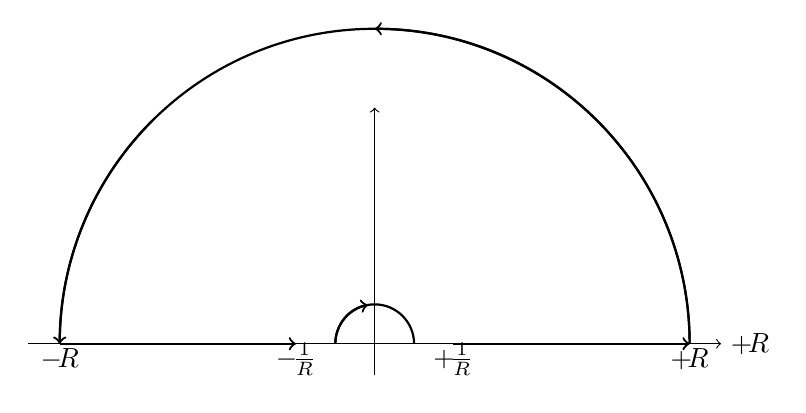
\begin{tikzpicture}[scale=2]
  % Axes
  \draw[->] (-2.2,0) -- (2.2,0) node[right] {$+$\!$R$};
  \draw[->] (0,-0.2) -- (0,1.5);

  % Semicircular arc (upper half-plane)
  \draw[thick, <-] (-2,0) arc (180:135:2);
  \draw[thick] (-2,0) arc (180:0:2);
  \draw[thick, <-] (0,2) arc (90:0:2);
  
  % Small semicircle around origin
  \draw[thick] (-0.25,0) arc (180:0:0.25);
  \draw[thick,->] (-0.25,0) arc (180:100:0.25);

  % Arrows along real axis
  \draw[thick, ->] (-2,0) -- (-0.5,0);
  \draw[thick, ->] (0.5,0) -- (2,0);

  % Labels
  \node at (-2, -0.1) {$-\!R$};
  \node at (-0.5, -0.1) {$-\!\frac{1}{R}$};
  \node at (0.5, -0.1) {$+\!\frac{1}{R}$};
  \node at (2, -0.1) {$+\!R$};
\end{tikzpicture}\]
Prove that 
\[\int_{\Gamma_R}(\frac{e^{iz}}{z} - \frac{1}{z})\,dz = 0.\]
\begin{solution}
    Since $\Gamma_R$ is closed, it suffices, by Cauchy's theorem, to show that $\frac{e^{iz}}{z} - \frac{1}{z}$ is entire on $D_{R + 1}(0).$ Clearly, The function $\in H(D_{R + 1}(0) \sm \{0\}).$ We will show that if we define 
    \[f(z)  = \begin{cases}
        \frac{e^{iz}}{z} - \frac{1}{z}, \quad z\neq 0\\
        i, \qquad \qquad z = 0
    \end{cases},\] then $f$ is continuous at $0$ since
    \[\lim_{z\to 0} f(z) = \lim_{z\to 0} \frac{1}{z}\sum_{n=0}^\infty \frac{(iz)^n}{n!} - \frac{1}{z} = i.\] Since we forgive singularities, we have that $f \in H(D_{R + 1}(0)).$ and so 
    \[\int_{\Gamma_R}(\frac{e^{iz}}{z} - \frac{1}{z}) \, dz = \int_{\Gamma_R}f(z)\, dz = 0.\]
\end{solution}


\newpage
\section*{Problem 2}
\begin{problem}
    Suppose that $\gamma_R(\theta) = Re^{i\theta}, \quad \theta \in [0, \pi]$ is the upper semicricle arc. Show that 
    \[\lim_{R\to \infty}\int_{\gamma_R} \frac{e^{iz}}{z}\,dz = 0\]
\end{problem}
\begin{figure}[H]
    \centering
    \includegraphics[width=0.5\linewidth]{Images/non-assmnet.png}
\end{figure}
\begin{solution}
Consider the paths in the picture above, where $\gamma_R^{(1)}, \gamma_R^{(3)}$ are the small pizza slices and $\gamma_R^{(2)}$ is the big pizza slice. Thus, 
\begin{align*}
    \left|\int_{\gamma_R} \frac{e^{iz}}{z}\, dz\right| &\leq \left|\int_{\gamma_R^{(2)}} \frac{e^{iz}}{z}\, dz\right| + 2\left|\int_{\gamma_R^{(1)}} \frac{e^{iz}}{z}\, dz\right|\\
    &\leq \text{arclength}\big[\gamma_R^{(2)}\big]\max_{z \in \gamma_R^{(2)}}(|\frac{e^{iz}|}{|z|}) + 2\cdot \text{arclength}\big[\gamma_R^{(1)}\big]\max_{z \in \gamma_R^{(1)}}(|\frac{e^{iz}|}{|z|})\\
    &\leq \pi R \frac{1}{R}\max_{z \in \gamma_R^{(2)}}(|{e^{iz}|}) + \epsilon R \frac{1}{R}\max_{z \in \gamma_R^{(1)}}(|{e^{iz}|})\\
    &= \pi \max_{y \in \gamma_R^{(2)}}({e^{-y}}) + \epsilon \max_{y \in \gamma_R^{(1)}}({e^{-y}})\\
    &= \pi {e^{-R\sin(\frac{\epsilon}{2})}} + \epsilon \\
    &\to \epsilon
\end{align*}

\end{solution}
\newpage

\section*{Problem 3}
\begin{problem}
    Prove that if $\Tilde{\gamma}_R = \frac{1}{R}e^{i\theta},$ $\theta \in [0, \pi],$ then 
    \[\lim_{R\to \infty} \int_{\Tilde{\gamma}_R}(\frac{e^{iz}}{z} - \frac{1}{z}) \, dz = 0 \]
\end{problem}
\begin{solution}
    Again, we estimate
    \begin{align*}
      \left|\int_{\Tilde{\gamma}_R}(\frac{e^{iz}}{z} - \frac{1}{z}) \, dz\right|  &\leq \text{arclength}\big[\Tilde{\gamma}_R\big]\max_{z \in \Tilde{\gamma}_R}(\frac{|e^{iz}|}{|z|} - \frac{1}{|z|})\\
      &= \frac{\pi}{R} \max_{z = \frac{1}{R}}(z + \frac{1}{2}z^2 + \dots)\\
      &\to 0
    \end{align*}
\end{solution}

\newpage
\section*{Problem 4}
\begin{problem}
    Prove that $\int_{-\infty}^\infty \frac{\sin(x)}{x}\, dx = \pi.$
\end{problem}
\begin{solution}
By symmetry, 
\[\int_{-R}^R \frac{\cos(x)}{x}\,dx =  \int_{-R}^R \frac{1}{x}\, dx = 0.\] Thus, by the previous part, we can say that in the limit,
\begin{align*}
    i\int_{-R}^R \frac{\sin(x)}{x}\, dx &= \int_{-R}^R \frac{\cos(x) + i\sin(x)}{x}- \frac{1}{x}\, dx\\
    &= \int_{-R}^R \frac{e^{ix}}{x} - \frac{1}{x}\, dx\\
    &= \int_{\Gamma_R}\frac{e^{iz}}{z} - \frac{1}{z}\, dz - \int_{\gamma_R}\frac{e^{iz}}{z} - \frac{1}{z}\, dz\\
    &= \int_{\gamma_R} \frac{1}{z}\,dz\\
    &= \int_0^\pi \frac{1}{Re^{i\theta}}Rie^{i\theta}\\
    &= i\pi,
\end{align*}
and thus 
\[\int_{-R}^R \frac{\sin(x)}{x}\, dx = \pi\]
    
\end{solution}

\newpage
\section*{Problem 5}
\begin{problem}
    Verify the Cauchy-Riemann equations for 
    \[f(z) = e^{z^2}\]
\end{problem}
\begin{solution}
    ($\frac{\partial u}{\partial x} = \frac{\partial v}{\partial y}$) Note that 
    \[e^{z^2} = e^{2z}= e^{2x + 2iy} = e^{2x}(\cos(2y) + i\sin(2y)) = e^{2x}\cos(2y) + ie^{2x}\sin(2y).\] Thus
    \begin{align*}
      \frac{\partial u}{\partial x}  &=   2e^{2x}\cos(2y)\\
      &= e^{2x}(2\cos(2y))\\
      &= \frac{\partial v}{\partial y}
    \end{align*}
    and 
    \begin{align*}
        \frac{\partial v}{\partial x} &= 2e^{2x}\sin(2y)\\
        &= -(-2e^{2x}\sin(2y))\\
        &= -\frac{\partial u}{\partial y}
    \end{align*}
\end{solution}

\newpage
\section*{Problem 6}
\begin{problem}
    Suppose that $a,b \in \bbC$ with $|a| < r < |b|$ and 
    \[\gamma(\theta) = re^{i\theta}, \quad \theta \in [0, 2\pi].\] Evaluate 
    \[\int_\gamma \frac{1}{(z - a)(z-b)}\, dz.\]
\end{problem}
\begin{solution}
    Consider the function
    \[f(z):= \begin{cases}
        \frac{1}{(z - a)(z-b)} - \frac{1}{(z-a)(a-b)}, \quad z\neq a\\
        \frac{-1}{(a-b)^2}, \qquad \qquad z = a
    \end{cases}\]
    Note that 
\begin{align*}
    \lim_{z\to a} f(z) &= \lim_{z\to a}\frac{1}{(z - a)(z-b)} - \frac{1}{(z-a)(a-b)}\\
    &= \lim_{z\to a} \frac{1}{z-a}\left[\frac{1}{z-b} - \frac{1}{a-b}\right]\\
    &= \lim_{z\to a} \frac{1}{z-a}\left[\frac{a-b - z + b}{(z-b)(b-a)}\right]\\
    &= \lim_{z\to a} \frac{-1}{(z-b)(a-b)}\\
    &= \frac{-1}{(a-b)^2}
\end{align*}. Thus, $f$ is continuous on $z = a.$ Moreover, there exists some $R$ such that $|r| < R < b,$ and thus $f\in H(D_R(0))$ since it forgives $z = a.$ Since $\gamma$ is closed, we have by Cauchy that 
\[\int_\gamma \frac{1}{(z - a)(z-b)} - \frac{1}{(z-a)(a-b)}\, dz = \int_\gamma f(z)\,dz = 0.\] Thus, it suffices to calculate 
\[\frac{1}{a-b}\int_\gamma \frac{1}{z - a}\,dz = \frac{1}{a-b}2\pi i.\] Thus, 
\[\int_\gamma \frac{1}{(z-a)(z-b)}\, dz = \frac{2\pi i}{b-a}\]
\end{solution}

\newpage
\section*{Problem 7}
\begin{problem}
    Suppose $f(z)$ is a nonconstant entire function. Prove that the range of $f$ is dense in $\bbC.$
\end{problem}
\begin{solution}
    Let $z_0\in \bbC.$ Suppose there exists some $r>0$ such that $f(z)\notin B_r(z)$ for any $z\in \bbC.$ Define 
    \[g(z) = \frac{1}{f(z) - z_0}.\] Note that $g \in H(\bbC).$ Note that 
    \[|g(z)| = \frac{1}{|f(z) - z_0|} < \frac{1}{r}.\] Thus, $g(z)$ is constant and so $f(z) - z_0$ is constant and thus $f$ is constant. A contradiction.
\end{solution}

\end{document}